\documentclass[10pt,a4paper]{article}

\usepackage[utf8]{inputenc}
\usepackage[T1]{fontenc}
\usepackage[english]{babel}
\usepackage[a4paper,left=10mm,right=11mm,top=10mm,bottom=10mm]{geometry}
\usepackage{xcolor}
\usepackage{graphicx}
\usepackage{tabularx}
\usepackage{array}
\usepackage{enumitem}
\usepackage{hyperref}

\IfFileExists{fontawesome5.sty}{
  \usepackage{fontawesome5}
  \newcommand{\IconMail}{\faIcon{envelope}}
  \newcommand{\IconPhone}{\faIcon{phone}}
  \newcommand{\IconLocation}{\faIcon{map-marker-alt}}
  \newcommand{\IconProfile}{\faIcon{linkedin}}
}{
  \newcommand{\IconMail}{@}
  \newcommand{\IconPhone}{T}
  \newcommand{\IconLocation}{\textbullet}
  \newcommand{\IconProfile}{in}
}

\definecolor{CVPrimary}{HTML}{1d1f27}
\definecolor{CVAccent}{HTML}{03a883}
\definecolor{CVText}{HTML}{111010}
\definecolor{CVMuted}{HTML}{2d3c39}
\definecolor{CVSoft}{HTML}{e1e3e8} 


\hypersetup{
  pdftitle={Natalie Böhm -- Networking Presales Consultant -- HPE},
  pdfauthor={Natalie Böhm},
  pdfsubject={Networking Presales Consultant},
  colorlinks=true,
  urlcolor=CVText,
  linkcolor=CVText
}

\renewcommand{\familydefault}{\sfdefault}
\pagestyle{empty}
\setlength{\parindent}{0pt}
\setlength{\parskip}{0pt}
\setlist[itemize]{leftmargin=4mm,topsep=0.6mm,itemsep=0.25mm,parsep=0mm}

\newcommand{\sidebarsection}[1]{%
  \vspace{2mm}%
  {\normalsize\bfseries\textcolor{CVPrimary}{\MakeUppercase{#1}}}\par
  \vspace{0.8mm}{\color{CVAccent}\rule{\linewidth}{0.6pt}}\vspace{1.1mm}
}

\newcommand{\mainsection}[1]{%
  \vspace{2mm}%
  {\large\bfseries\textcolor{CVPrimary}{\MakeUppercase{#1}}}\par
  \vspace{0.8mm}{\color{CVAccent}\rule{\linewidth}{0.6pt}}\vspace{1.2mm}
}

\newcommand{\sideitem}[2]{%
  {\bfseries #1}\par
  {\small #2}\par\vspace{1.2mm}
}

\newcommand{\contactitem}[2]{%
  \makebox[5mm][c]{\textcolor{CVPrimary}{#1}}%
  \hspace{1mm}%
  \begin{minipage}[t]{\dimexpr\linewidth-6mm\relax}
    {\small #2}
  \end{minipage}\par\vspace{1.2mm}
}

\newcommand{\entry}[4]{%
  \begin{tabularx}{\linewidth}{@{}>{\raggedright\arraybackslash}p{0.13\linewidth}@{\hspace{2.5mm}}X@{}}
    {\small\textcolor{CVMuted}{#1}} &
    {\bfseries #2}\hfill{\small\textcolor{CVMuted}{#3}}\par
    #4
  \end{tabularx}\vspace{1.2mm}
}

\newcommand{\compactentry}[3]{%
  {\bfseries #1}\hfill{\small\textcolor{CVMuted}{#2}}\par
  #3\par\vspace{1.7mm}
}

\newcommand{\tag}[1]{%
  \begingroup
  \setlength{\fboxsep}{1.4pt}%
  \colorbox{CVSoft}{\scriptsize\textcolor{CVPrimary}{#1}}%
  \endgroup\hspace{0.7mm}%
}

\begin{document}
\color{CVText}

\begin{minipage}[t]{0.26\textwidth}
  \vspace{0pt}
  \setlength{\fboxsep}{3mm}%
  \colorbox{CVSoft}{%
    \begin{minipage}[t][\dimexpr\textheight-2\fboxsep-5mm\relax]{\dimexpr\linewidth-2\fboxsep\relax}
      \vspace{1mm}
      {\centering
      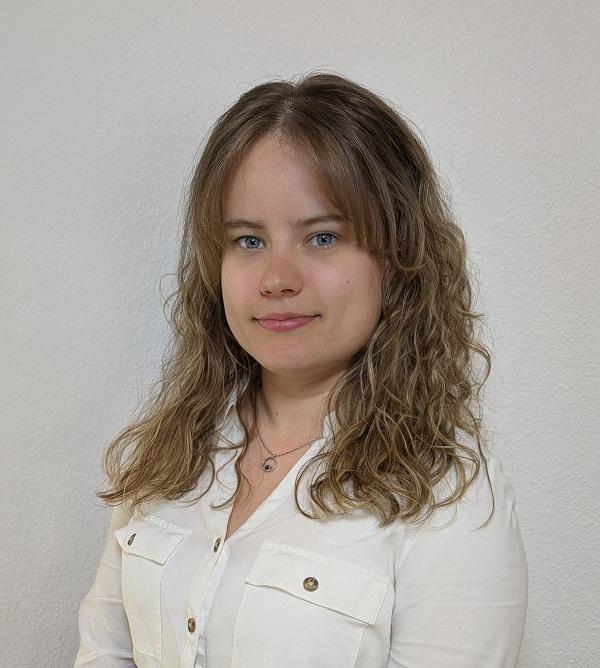
\includegraphics[width=3.55cm,height=4.35cm,keepaspectratio]{Bewerbungsbild.jpg}\par}
      \vspace{3mm}

      
      \sidebarsection{Contact}
      \contactitem{\IconMail}{{\footnotesize\href{mailto:kontakt@natalieboehm.de}{kontakt@natalieboehm.de}}}
      \contactitem{\IconPhone}{+49 1522 1746238}
      \contactitem{\IconLocation}{Aalen}
      \contactitem{\IconProfile}{{\footnotesize\href{https://www.linkedin.com/in/natalieboehm2}{@natalieboehm2}}}

      \sidebarsection{Skills}
      \small
      \textbf{Networking \& Infrastructure}\par
      DNS, Network Troubleshooting, Linux, Podman, Kubernetes (basics)\par\vspace{1.1mm}
      \textbf{NetOps \& Automation}\par
      Python, Ansible, Docker, CI/CD, Azure\par\vspace{1.1mm}
      \textbf{AI \& Monitoring}\par
      LLMs, PyTorch, Splunk, Elastic, Power BI, Pandas\par\vspace{1.1mm}
      \textbf{Software}\par
      Python, Java, C\#, SQL, Django, Testing\par\vspace{1.1mm}
      \textbf{Communication}\par
      Technical presentations,\par
      stakeholder communication,\par
      process optimization,\par
      teamwork

      \sidebarsection{Languages}
      German: Native\par
      English: C1\par
      French: B2\par
      Spanish: B2\par
      Korean: A2

      \sidebarsection{International}
      Internship semester in Poland with Bosch\par
      Semester abroad in Korea

      \sidebarsection{Certificates}
      AI Leadership\par
      {\small NextEducation}

      \sidebarsection{Interests}
      Dancing\par
      Martial arts\par
      Hackathons\par
    \end{minipage}%
  }
\end{minipage}
\hfill
\begin{minipage}[t]{0.705\textwidth}
  \vspace{0pt}
  {\fontsize{25}{28}\selectfont\bfseries\color{CVAccent} Natalie Böhm}\par
  \vspace{1mm}
  {\Large\textcolor{CVPrimary}{HPE Networking Presales Consultant}}\par
  \vspace{2.5mm}
  {\small
    I combine a solid IT foundation in infrastructure and automation with a strong analytical mindset. Hands-on experience from Bosch, ZEISS and Selfnet lets me understand customer environments and recommend solutions that work.
IT is more than a career path to me -- it is an environment in which I
also engage privately and implement my own ideas.
  }\par

  \mainsection{Education}

  \entry{10/2024--09/2026}{M.Sc. Machine Learning \& Data Analytics}{Aalen University}{
    Focus: NLP, Deep Learning and Computer Vision\par
    Master's thesis: AI-based Signal Separation of Friedel Pairs in Crystallography
  }

  \entry{10/2021--09/2024}{B.Sc. Business Information Systems}{DHBW / Bosch Stuttgart}{
    Dual degree programme with a focus on Application Management\par
    Bachelor's thesis: Application and Evaluation of Domain Adversarial Training for Parking Assistants
  }

  \entry{09/2012--06/2021}{Abitur}{Nellenburg-Gymnasium Stockach}{}

\mainsection{Professional Experience}
  \entry{09/2026 -- present}{Research Associate}{Aalen University, Institute of Drive Technology}{
    Development of a data-driven method for predicting the remaining useful life of band saws\par
    Setup of measurement technology and sensor data acquisition\par
    \tag{Python}\tag{Condition Monitoring}\tag{Sensor Technology}
  }
  \entry{04/2025--08/2026}{Working Student}{ZEISS SMT GmbH, Oberkochen}{
    Development of a reinforcement learning agent
      for solving industrial scheduling problems\par
      Monitoring and analysis of machine utilization
      to support data-based decisions\par
    \tag{Python}\tag{Reinforcement Learning}\tag{Scheduling}\tag{Elastic}
  }

  \entry{10/2024--03/2025}{Working Student}{Robert Bosch GmbH, Stuttgart-Feuerbach}{
    Improvement of asset management with RFID technologies\par Evaluation of an
    AI chatbot with internal tools for knowledge management; insights into
    industrial digitalization and data-driven process improvement\par
    \tag{GenAI Bots}\tag{Knowledge Management}\tag{Process Analysis}\tag{Scrum}
  }

  \entry{10/2021--09/2024}{Dual Student}{Robert Bosch GmbH, Stuttgart-Feuerbach}{
    Rotation through the departments SIEM, Hadoop, internal consulting and Driving Experience with a focus on parking
    assistants\par
    \tag{Hadoop}\tag{Infrastructure}\tag{Splunk}\tag{Python}\tag{Linux}\tag{Azure}
  }

  \mainsection{Engagement \& Projects}

  \compactentry{Selfnet e.\,V. -- Infrastructure and Development}{since Bachelor's studies}{
    Second board assessor, development of the membership management system, hardware maintenance,
    DNS administration, member support for network issues\par
    \tag{Django}\tag{Python}\tag{Podman}\tag{DNS}\tag{Kubernetes basics}
  }

  \compactentry{Private Infrastructure}{private}{
    Automated configuration and administration of own systems with Ansible
    (Nextcloud, Home Assistant), use of LLMs, training of custom
    wake-word detection models\par
    \tag{Ansible}
  }

  \compactentry{InnoConsult e.\,V. -- Consulting and Project Work}{during Master's studies}{
    Event management, design thinking workshops, development of marketing strategies for startups.
  }
\end{minipage}

\end{document}